% ------------------------------------------------------------------------ %
% !TEX encoding = UTF-8
% !TEX TS-program = pdflatex
% !TEX root = RASD.tex
% !TEX spellcheck = en-EN
% ------------------------------------------------------------------------ %
%
%
% ------------------------------------------------------------------------ %
% 	PREAMBLE
% ------------------------------------------------------------------------ %
%
\documentclass
	[12pt,	
	a4paper,		%
	twoside,		% fronte-retro
	openany,
	titlepage,% 	% nuova pagina dopo il titolo (necessario per frontespizio)
	]{book}
%
% ------------------------------------------------------------------------ %
%
\usepackage[T1]{fontenc}		% codifica di output
%
\usepackage[utf8]{inputenc}		% codifica di input; anche [latin1] va bene
%
\usepackage[italian,english]{babel}	% languages
%
\usepackage{csquotes}
%
\usepackage{microtype}		% micro-tipografia
%
\usepackage{lmodern}
%
\usepackage{pdflscape}
%
% ------------------------------------------------------------------------ %
%
% 	LAYOUT - MARGINS - BINDING
%
% -- MANUAL (PoliMi settings)
\usepackage{geometry}
\geometry{verbose,	% verbose = displays the parameter results on the terminal
	top=43mm,		% upper margin (PoliMi=43mm)
	bottom=44mm,	% bottom margin (PoliMi=44mm)
	inner=37mm,		% inner margin (PoliMi=41mm)
	outer=37mm,		% outer margin (PoliMi=32mm)
%	bindingoffset=5mm,	% binding margin
	heightrounded}
%
% ------------------------------------------------------------------------ %
%
\usepackage{changepage,calc}                 % centra il frontespizio
%
\usepackage{emptypage}		% pagine vuote senza testatina e piede di pagina
%
\usepackage{indentfirst}	% rientra il primo paragrafo di ogni sezione
%
\usepackage{booktabs}		% tabelle (\toprule, \midrule, \bottomrule)
%
\usepackage{tabularx}		% tabelle di larghezza prefissata
%
\usepackage{graphicx}		% immagini
%
\usepackage[figuresright]{rotating}	% tabelle a 90 gradi
%
\usepackage{subfig}			% sottofigure, sottotabelle
%
\usepackage{caption}		% didascalie
%
\usepackage{listings}		% codici
%
\usepackage[font=small]{quoting}	% citazioni
%
\usepackage{amsmath,amssymb}	% matematica
%
\usepackage{mathtools}		% matematica
%
\usepackage{amsthm}			% matematica
%
\usepackage[output-decimal-marker={,}]{siunitx}	% SI (con separatore decimale=virgola)
%
\usepackage[english]{varioref}		% riferimenti completi, con indicazione della pagina (\vref)
%
\usepackage{mparhack}	% finezze tipografiche (bug fixes di LaTeX)
%
\usepackage{relsize}			% make text larger or smaller than the surrounding text
% 				% \larger[i] \smaller[i]
%
% ------------------------------------------------------------------------ %
%
% 	BIBLIOGRAPHY
%
%
% biblatex package
%
% STILI di citazione:
% style=numeric-comp,	<-- ufficialmente richiesto dal PoliMi (numeri tra [ ])
% style=philosophy-modern,	<-- autore-anno (meno anonimo, pi� immediato e pi� elegante)
%
\usepackage[style=philosophy-modern,	% numeric-comp oppure philosophy-modern,
	hyperref,			% clickable references
	backref,			% link alle pagine in cui il riferimento � citato
	natbib, 			% mantiene compatibilit� con eventuali comandi natbib
	backend=biber,		% motore bibliografico (v. ArteLatex di Pantieri)
	defernumbers=true,	 	% riferimenti ordinati in ordine di comparsa
	]{biblatex}
%
\addbibresource{Bibliografia.bib}	% database bibliografico
%
% ------------------------------------------------------------------------ %
%
% Per generare effettivamente la bibliografia nel documento
% questa e` la sequenza di composizione:
% 1. si compone il documento con LATEX una prima volta;
% 2. si lancia il programma Biber premendo l�apposito pulsante dell�editor;
% 3. si compone il documento altre 2 volte con LATEX (ma anche 3, NdA)
% Tale sequenza deve essere ripetuta solo se vengono fatte modifiche/aggiunte
% al database bibliografico.
%
% ------------------------------------------------------------------------ %
%
\usepackage[dvipsnames]{xcolor}	% colori - 68 colori predefiniti:
% 								% http://en.wikibooks.org/wiki/LaTeX/Colors
%
\usepackage{lipsum}			% testo fittizio
%
\usepackage{eurosym}		% simbolo dell'euro
%
\usepackage{hyperref}		% collegamenti ipertestuali
\hypersetup{
    colorlinks = false,
    linkbordercolor = {white}
}
%
\usepackage{bookmark}		% gestione segnalibri del PDF
%
\usepackage{guit}			% simboli del Guit
%
\usepackage{fancyhdr}		% testatine e piede personalizzati
\pagestyle{fancy}
\fancyhead[LO,LE]{\slshape \leftmark}
\fancyhead[RE,RO]{\slshape \rightmark}
\fancyfoot[C]{\thepage}
\renewcommand{\chaptermark}[1]{\markboth{\MakeUppercase{\thechapter.\ #1}}{}}
\renewcommand{\sectionmark}[1]{\markright{\thesection.\ #1}}
\setlength{\headheight}{15pt}
%
\usepackage{colortbl}		% per colorare i filetti delle tabelle
%
\usepackage[footnote,		% acronym description in the footer
			smaller,		% smaller acronyms size
			]{acronym}		% acronyms
%
\usepackage{multirow}		% celle tabelle alte pi� di una riga
%
\usepackage{pdfpages}		% adding external pdf files
%
\usepackage[dvipsnames]{xcolor} %alloy
\usepackage{listings}
\usepackage{alloy-style}
%
\renewcommand{\thesection}{\thechapter.\Alph{section}}
%
% ------------------------------------------------------------------------ %
% 	BEGIN DOCUMENT
% ------------------------------------------------------------------------ %
%
\begin{document}
%
% ------------------------------------------------------------------------ %
% 	FRONTMATTER
% ------------------------------------------------------------------------ %
%
\frontmatter
%
% Frontispiece

\includepdf[pages={1}]{FrontMatter/Frontispiece.pdf}
%
\let\cleardoublepage\clearpage
%
\clearpage
\setcounter{page}{1}
\pagenumbering{Roman}
\tableofcontents
%
%\input{FrontMatter/Colophon}
%
%\input{FrontMatter/Thanks}
%
%\input{FrontMatter/Dedication}
%
%\input{FrontMatter/Indexes}
%
%\input{FrontMatter/SommarioAbstract}
%
% ------------------------------------------------------------------------ %
% 	MAINMATTER
% ------------------------------------------------------------------------ %
%
\mainmatter
%
% ------------------------------------------------------------------------ %
% !TEX encoding = UTF-8
% !TEX TS-program = pdflatex
% !TEX root = ../Project.tex
% !TEX spellcheck = en-EN
% ------------------------------------------------------------------------ %
%
% ------------------------------------------------------------------------ %
% 	CHAPTER TITLE
% ------------------------------------------------------------------------ %
%
\chapter{Introduction}
%
\label{cap:introduction}
%
% ------------------------------------------------------------------------ %
%
This document is the Requirement Analysis and Specification Document (RASD) of a mobile application called Travlendar+. The purpose of the document is to show the requirements and specification of the new application, considering various aspects like the stakeholders' needs, domain properties and constrains which the system-to-be is subject to.
%
% ------------------------------------------------------------------------ %
%
\section{Description of the given problem}
Travlendar+ is a mobile, calendar-based application that helps the user to manage his appointments and to a greater extent set up the trip to his destination, choosing the best means of transport depending on his needs. \\
Travlendar+ will choose the most suitable way to get the user to his destination between a large pool of options, considering public transportation, personal vehicles, locating cars or bikes of sharing services and walking to the destination. It will take account of weather, traffic, possible passengers if any, the user-set break times and the potential will to minimize the carbon footprint of the trip, always focusing on taking him on time to his scheduled appointments. \\
Eventually the user will be able to purchase the tickets he will use to reach his destination in-app. The great customizability is one of the main strengths of Travlendar+, being able to fully comply with the user needs. 
%
% ------------------------------------------------------------------------ %
%
\section{Definitions and Acronyms}
%
\subsection{Definitions}
\begin{itemize}
\item Application: it depends on context, but often it is referred to Travlendar+;
\item User: see 2.A - Actors;
\item Guest: see 2.A - Actors;
\item System: see Application;
\item Event: often used as a key word referring to the events the user can add on the calendar embedded in Travlendar+;
\item Trip: often used as a key word referring to the trips alternatives the system processes and suggests the user;
\item Dynamic event: Event whose location in time can be decided by the application on various factors;
\item Means of transport: often used as a key word referring to the means of transportation the user can choose in the settings of Travlendar+;
\item Private transports: often used to mean trains, planes and all private companies transports;
\item Shared means: used to mean cars and bicycles of car and bike sharing companies.
\end{itemize}
%
\subsection{Acronyms}
List of the acronyms used in this paper:
\begin{itemize}
\item RASD: Requirements analysis and specification document;
\item ETA: Estimated time of arrival, it's the time remaining to arrive to destination;
\item POI: Point of interest;
\item API: Application programming interface;
\item UI: User Interface.
\end{itemize}
%
% ------------------------------------------------------------------------ %
%
\section{Revision History}
\begin{itemize}
\item 29/10/2017 Version 1.0.0 - First complete drawing up of the RASD;
\item 18/11/2017 Version 1.0.1 - Fixed some grammatical errors;
\item 24/11/2017 Version 1.1.0 - Changed Sections 3.B.4 - Communication interfaces and 3.F.3 - Security;
\item 26/11/2017 Version 1.1.1 - Added some acronyms and modified requirement 34.
\end{itemize}
%
% ------------------------------------------------------------------------ %
%
\section{References}
Documents list:
\begin{itemize}
\item Mandatory Project Assignments.pdf
\item IEEE Std 830-1998 IEEE Recommended Practice for Software Requirements
Specifications
\item RASD sample from Oct. 20 lecture.pdf
\end{itemize}
Online sites list:
\begin{itemize}
\item http://alloy.mit.edu/alloy/documentation.html
\end{itemize}
%
% ------------------------------------------------------------------------ %
%
\section{Document Structure}
The paper is structured as follows:
\begin{itemize}
\item Chapter 1: Introduction to the document, including some information about its composition and the description of the problem;
\item Chapter 2: General description of the system functions and assumptions, together with information about the environment and the users;
\item Chapter 3: Detailed description of the functional, non functional requirements and constraints;
\item Chapter 4: System usage examples; 
\item Chapter 5: Specific modeling of system functions, abstract structure and usage;
\item Chapter 6: Formal analysis of the system and his functions using Alloy;
\item Chapter 7: Effort spent by the authors to draw up the document.
\end{itemize}
%
% ------------------------------------------------------------------------ %
%
\section{Used tools}
The tools used to create this document are:
\begin{itemize}
\item StarUML for UML mode;
\item Alloy Analyzer 4.2 for proving consistency of the model and to challenge it to find counterexamples for our assertions;
\item Github as version controller and to share documents;
\item LaTeX for typesetting this document;
\item Texmaker as editor
\item Draw.io to create sequence diagrams and state diagrams;
\item Signavio to create use case diagrams;
\item Photoshop for mockups.
\end{itemize}
%
% -----------------------------END------------------------------------- %

%
% ------------------------------------------------------------------------ %
% !TEX encoding = UTF-8
% !TEX TS-program = pdflatex
% !TEX root = ../Project.tex
% !TEX spellcheck = en-EN
% ------------------------------------------------------------------------ %
%
% ------------------------------------------------------------------------ %
% 	CHAPTER TITLE
% ------------------------------------------------------------------------ %
%
\chapter{Overall Description}
%
\label{cap:overalldescription}
%
% ------------------------------------------------------------------------ %
%
\section{Product Perspective}
Travlendar+ will be developed as a mobile application that relies on the use of Google maps and Google calendar APIs. \\
Its user interface will be composed by two main tabs, one with a calendar, to schedule user's events and the other one with a map to manage the movements of the user. \\
In the future will have a service of technical assistance via chat. \\
The application will not provide any API for integration with other systems.
\\
\\
***************************** Further details on the shared phenomena and a domain model (class diagrams and statecharts)
%
% ------------------------------------------------------------------------ %
%
\section{Product Functions}
******************************************** Requirements
%
% ------------------------------------------------------------------------ %
%
\section{User Characteristics}
The user of the system-to-be is every person who wants to schedule appointments in a calendar and manage his movements from a location to another at the same time.
Users can use it to organize work events, but also include family or spare time events. The application doesn't have any age limit, or any other restriction applied to the user characteristic. In order to make the application work without limitation the user need to have access to the Internet, but he can access and modify the calendar offline.
%
% ------------------------------------------------------------------------ %
%
\section{Assumptions, Dependencies, Constraints}
********************************************* Domain assumptions
\\
Regulatory policy:
The System asks the User for the permission to acquire, store and use his personal data, and informs him that won't take any responsibility for a use of it that doesn't complies with the local laws and policies, by means of the User agreement's acceptance.
The System under request of the User must delete all his personal data.
%
% -----------------------------END------------------------------------- %
%
% ------------------------------------------------------------------------ %
% !TEX encoding = UTF-8
% !TEX TS-program = pdflatex
% !TEX root = ../Project.tex
% !TEX spellcheck = en-EN
% ------------------------------------------------------------------------ %
%
% ------------------------------------------------------------------------ %
% 	CHAPTER TITLE
% ------------------------------------------------------------------------ %
%
\chapter{Specific Requirements}
%
\label{cap:specificrequirements}
%
%
**************************************************************************************************************************************************************************************************************************************** \\
More details on all aspects in Section 2 if they can be useful for the development team
%
%------------------------------------------------------------------------ %
\section{External Interface Requirements}
% ------------------------------------------------------------------------ %
\subsection{User interfaces}
The application will be developed as a mobile application for the main mobile operative systems (iOS and Android).
Its user interface will appear the same to all users, and must be user-friendly and intuitive. To show how the application will look like some mockups of the user interface are present in the document (mockups are realized for iOS operative system).
\begin{center}
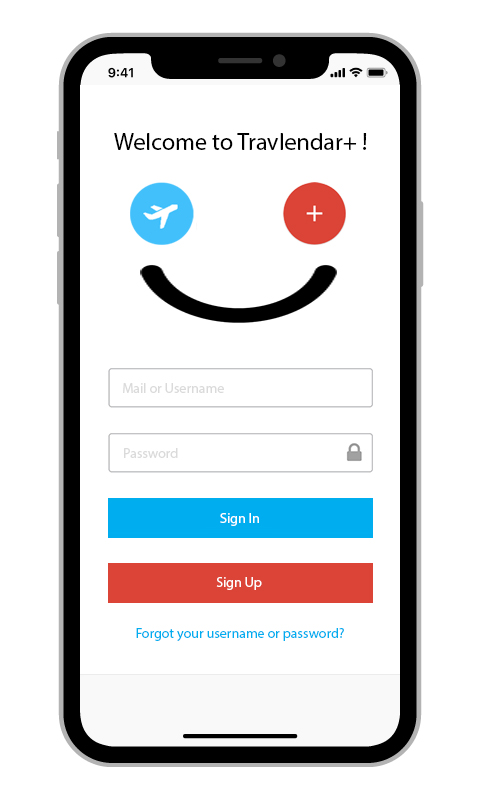
\includegraphics[scale=2.4]{MainMatter/images/ui/login}
\captionof{figure}{Mockup of the login screen}
\end{center}
After downloading the application from the store of the OS. At the first start if the user is not registered, so it is a guest yet, he must sign up. Otherwise he can log in. If he is signing up he will see the registration screen.
\begin{center}
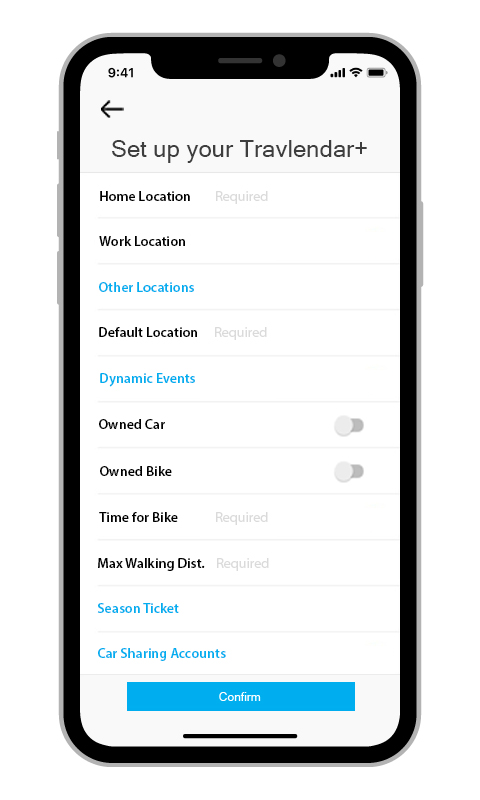
\includegraphics[scale=2.4]{MainMatter/images/ui/firstsetup}
\captionof{figure}{Mockup of the first configuration screen}
\end{center}
The first time the user signs in, the application shows the first setup screen where the user has to insert all his preferences. The light blue texts open other screen where more are given for the specific setting. \\\
Once the application is configured, the first screen that will appear to the user at each startup is the main screen that shows up a calendar, where he can add his events.
\begin{center}
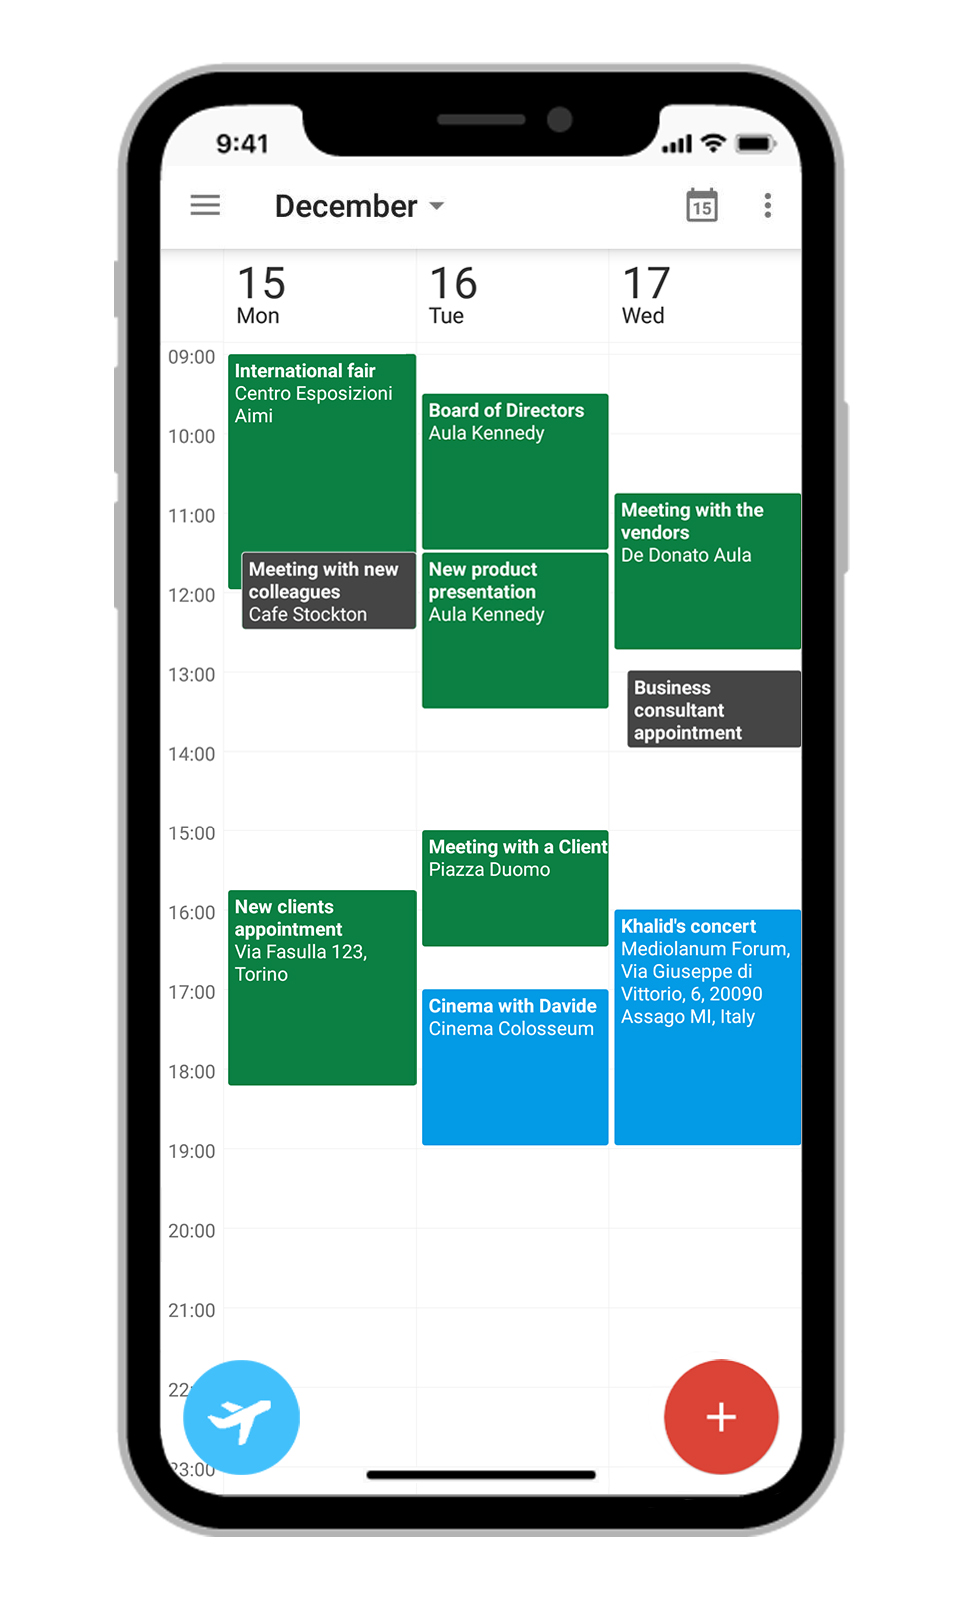
\includegraphics[scale=1.2]{MainMatter/images/ui/calendar}
\captionof{figure}{Mockup of the main screen (calendar)}
\end{center}
The events are the ones in green or blue, some event are not coloured cause are overlapped with others or the user cannot phisically arrive on time for them (the user chooses what event is primary and the application considers it to organize the trips. When the user chooses to add an event pressing the "Add Event" button on the bottom right corner (the red one with a cross on it), the application shows a screen where he can insert the details of it.
\begin{center}
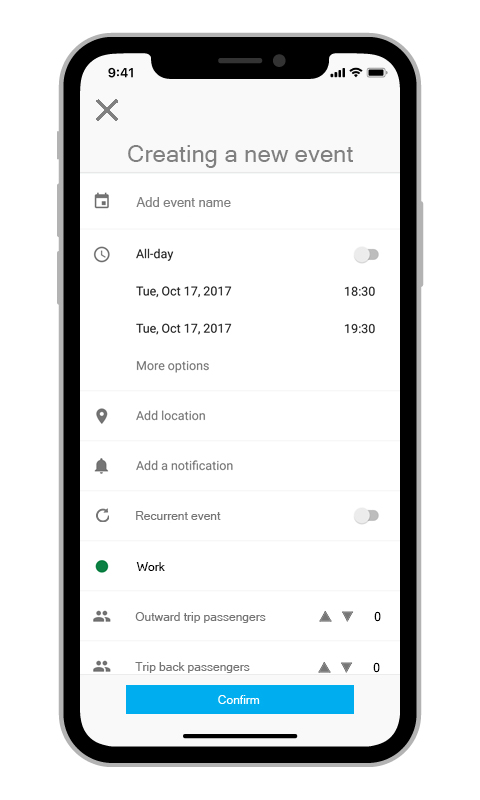
\includegraphics[scale=2.4]{MainMatter/images/ui/newevent}
\captionof{figure}{Mockup of the screen that appears to the user when he has to add an event}
\end{center}
When the main screen is showed by the application, to check the trips between home and an event, or between two events, the user can press the "Trips" button on the bottom left side of the screen (the light blue one with a plane on it) and the main screen will change to show the trips and all the confirmed events will become black and white.
\begin{center}
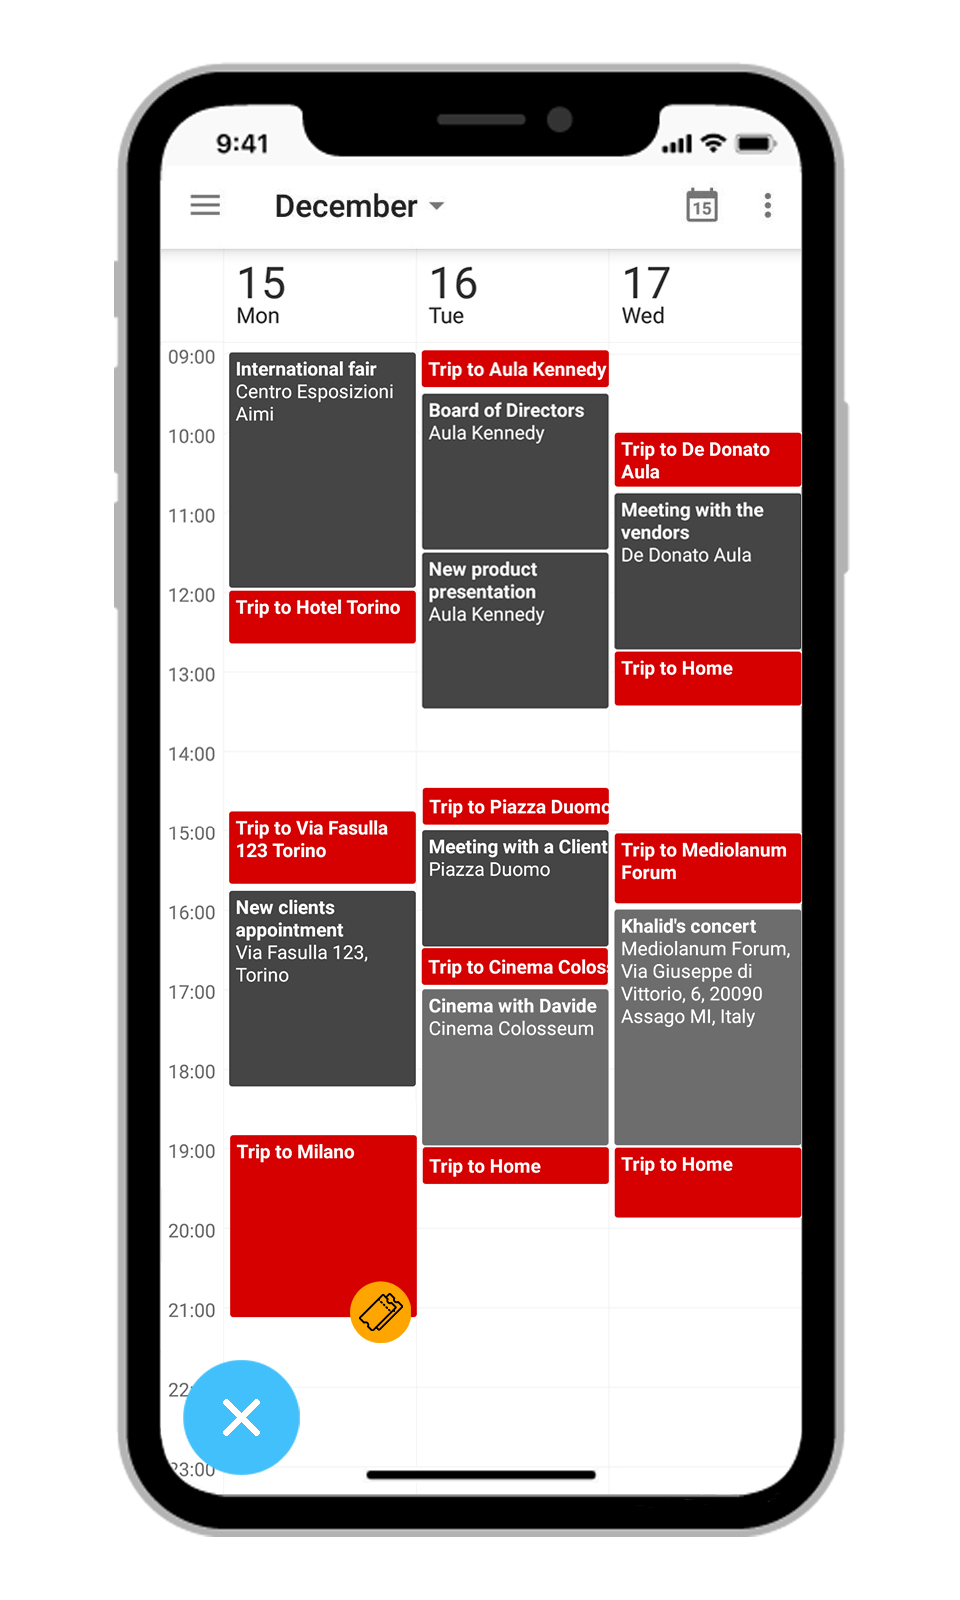
\includegraphics[scale=1.2]{MainMatter/images/ui/tripsscreen}
\captionof{figure}{Mockup of the screen that contains all the trips computed by the application for the user}
\end{center}
When the user taps on a trip he can check the details of it. If a trip presents an orange icon with some tickets on it, the user have to buy some tickets to complete the trip.
\begin{center}
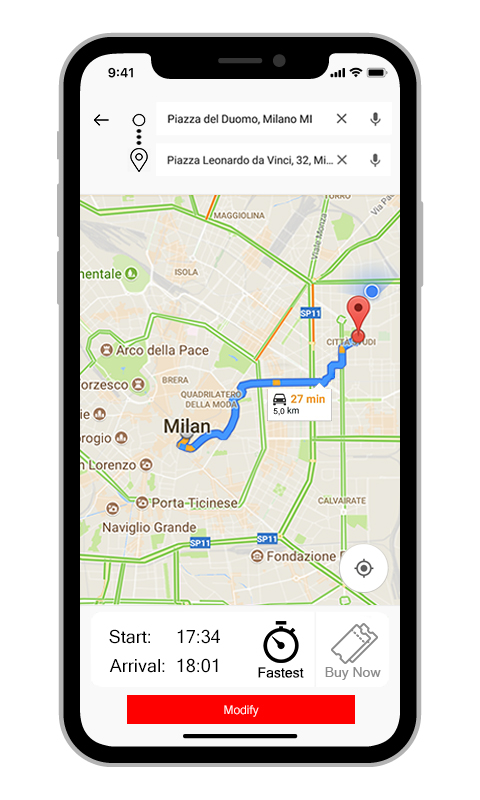
\includegraphics[scale=2.4]{MainMatter/images/ui/journeydetails}
\captionof{figure}{Mockup of the screen that shows the details of a trip}
\end{center}
This screen shows the trip details: the route, the ETA, the time of departure, the time of arrival, the type of trip selected. If some tickets are needed the "Buy Now" button with the tickets on it is grey, but black and it will be clickable. The "Buy Now" is juxtaposed with the "Sharing" button if the trip include some section in which car sharing or bike sharing are used; clicking on the "Bike sharing" or "Car sharing" button will show up a screen with the cars and bike around the user of the various local sharing service. \\
If an user wants to modify a trip, he just have to press "Modify" button and a screen will appear when he can change the trip options.
\begin{center}
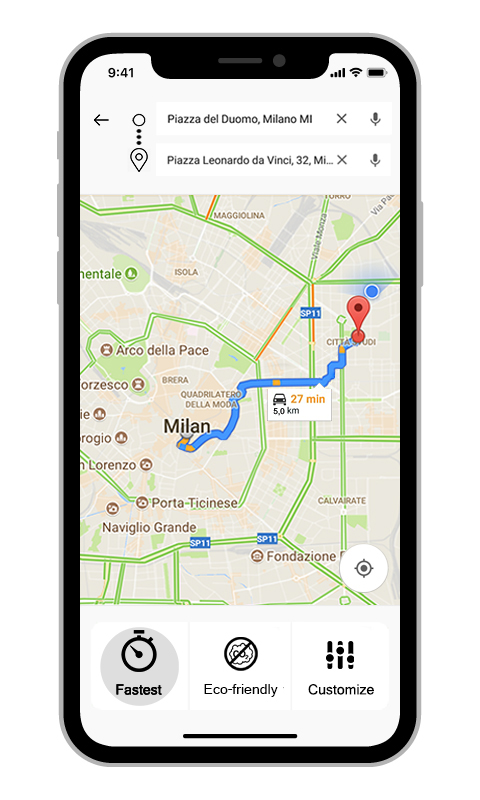
\includegraphics[scale=2.4]{MainMatter/images/ui/journeychoose}
\captionof{figure}{Mockup of the screen where the user can change the trip options}
\end{center}
The system select by default the fastest trip options, but the user can change them. It is also possible to choose a trip that minimize the carbon footprint.
\\
\\
When the application need to communicate messages to the user, while it’s open and the screen is turned on, it will show a pop up, otherwise it will send a push notification to the user.
%
\subsection{Hardware interfaces}
The main hardware interface used by the system is the GPS, it's used in order to correctly position the user in the map. Since the application uses the internet connection, all the hardware required to connect to the internet will be hardware interface for the system.
%
\subsection{Software interfaces}
The mobile application is made up using mainly two Google APIs: Google Maps and Google Calendar. It relies also on other APIs: one for the weather forecast and one for each car sharing, bike sharing service and for the public mobility.
It is developed for the use on the two most common mobile operating systems: Android and iOS.
%
\subsection{Communication interfaces}
The application communicates with the server using the protocol HTTP (port 80).
%------------------------------------------------------------------------ %
\section{Functional Requirements}
******************************************************************************************************************************************************************************************************* \\
Definition of use case diagrams, use cases and associated sequence/activity diagrams
% ------------------------------------------------------------------------ %
\subsection*{Use case description}
In this section some use cases will be described. These use cases can be
derived from the scenarios and the use case diagram.
%
\begin{center}
\def\arraystretch{1.25}
  \begin{tabular}{ | l | p{0.65\textwidth} | }
    \hline
    Name & Sign up \\ \hline
    Primary Actor & Guest \\ \hline
    Preconditions & The guest wants to register to “Travlendar+” \\ \hline
    Postconditions & Guest's informations are stored in the “Travlendar+” server and locally on the device. The Guest can sign in to use the application, becoming a user \\ \hline
    Flow of events  & 1.	The guest opens the application for the first time \\
					& 2.	The system shows the Login screen to the guest \\
					& 3.	The Guest clicks on “Sign Up” \\
					& 4.	The System shows to the Guest the Registration page \\
					& 5.	The guest inserts his personal details (name, surname, …) and his trip preferences (important addresses, owned car, season ticket, …) \\
					& 6.	The guest reads and accepts the user agreement \\
					& 7.	The guest taps on “Confirm” \\
					& 8.	The system check the correctness of the data and sends an email and a sms with a verification link \\
					& 9.	The guest confirms his registration clicking on one of the verification links \\
					& 10.	The guest is now registered and becomes a User of “Travlendar+” \\
					& 11.	The system shows to the user the Main screen (Calendar) of the application \\ \hline    
    Exceptions  & 1.	One or more fields of the Registration page are not well formed \\
				& 2.	Username is already in use \\
				& 3.	Email is already in use \\
				& 4.	The verification link is expired (after 24 hours)\\ \hline
  \end{tabular}
\captionof{table}{Use case for sign up}
\end{center}

\begin{center}
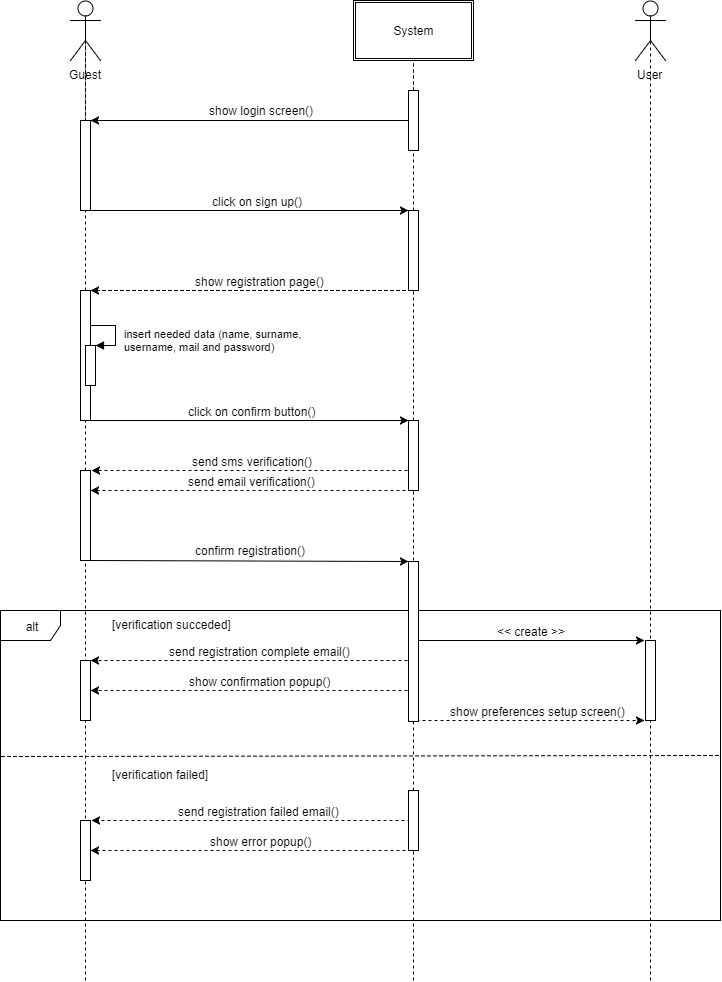
\includegraphics[scale=0.55]{MainMatter/images/sequencediagrams/signup}
\captionof{figure}{Sequence diagram of sign up use case}
\end{center}

\begin{center}
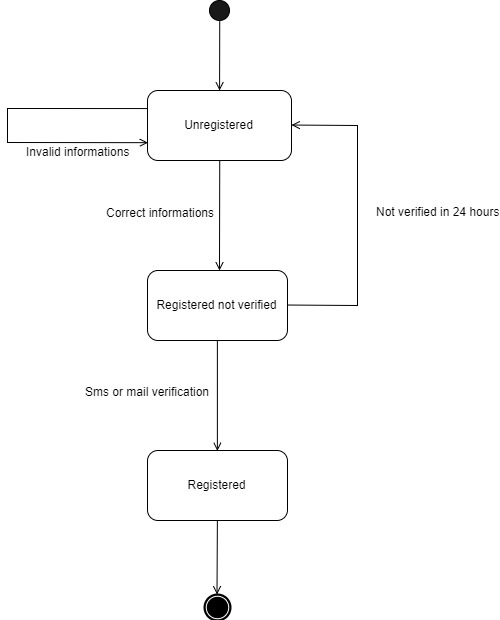
\includegraphics[scale=0.8]{MainMatter/images/statecharts/signup}
\captionof{figure}{Statechart of sign up process}
\end{center}

\begin{center}
\def\arraystretch{1.25}
  \begin{tabular}{ | l | p{0.65\textwidth} | }
    \hline
    Name & Sign in \\ \hline
    Primary Actor & Guest \\ \hline
    Preconditions & The guest wants to sign in to use “Travlendar+”. He is actually an user of the application because he has a valid account for it \\ \hline
    Postconditions & The guest is now logged into the system becoming an user \\ \hline
    Flow of events  & 1.	The guest opens the application \\
					& 2.	The system shows to the guest the Login screen \\
					& 3.	The guest inserts account credentials (username and password) \\
					& 4.	The guest taps on “Sign In” \\
					& 5.	The system checks if the credentials  are present in the database \\
					& 6.	The guest is now logged and becomes an user \\
					& 7.	The system shows to the user the Main screen of the application \\ \hline    
    Exceptions  & 1.	One or more fields of the Login page are not well formed \\
    			& 2.	Username is not present in the database \\
				& 3.	The password associated to the username is incorrect \\ \hline
  \end{tabular}
\captionof{table}{Use case for sign in}
\end{center}

\begin{center}
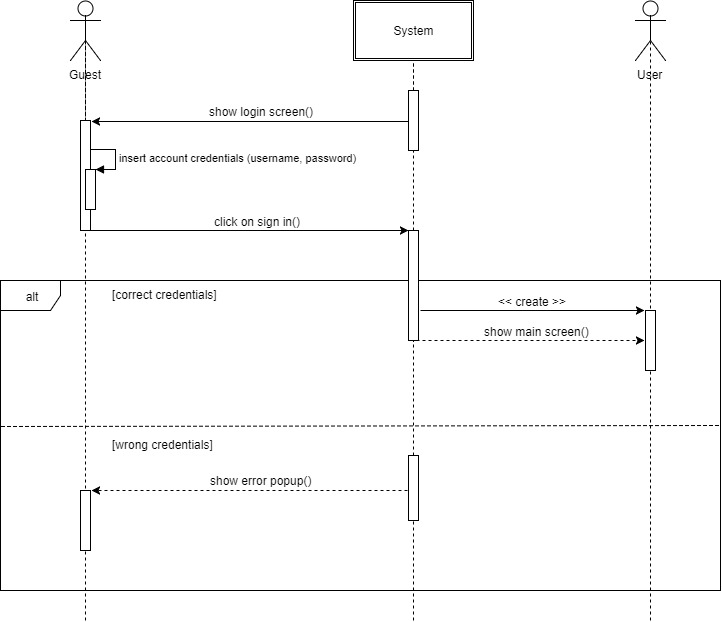
\includegraphics[scale=0.55]{MainMatter/images/sequencediagrams/signin}
\captionof{figure}{Sequence diagram of sign in use case}
\end{center}


\begin{center}
\def\arraystretch{1.25}
  \begin{tabular}{ | l | p{0.65\textwidth} | }
    \hline
    Name & Add event to calendar \\ \hline
    Primary Actor & User \\ \hline
    Preconditions & The user wants to add an event to the calendar of his application. He is already logged in into the service and the system is showing the calendar \\ \hline
    Postconditions & The event is added to the calendar and stored in the database, the system computes the round trip from the location of the event and shows again the calendar to the user \\ \hline
    Flow of events  & 1.	The user taps on “Add Event” (the red button with a white cross) \\
					& 2.	The system shows the Add Event screen \\
					& 3.	The user inserts the details in the requested fields \\
					& 4.	The user clicks on “Confirm” \\
					& 5.	The system adds the event to the calendar and shows the updated Main screen to the user \\
 \hline    
    Exceptions  & 1.	The event overlaps with another one \\
				& 2.	The event overlaps with user’s lunch \\
				& 3.	One or more field are not well formed \\
				& 4.	The user cannot arrive in time for the event \\
 \hline
  \end{tabular}
\captionof{table}{Use case for add event}
\end{center}

\begin{center}
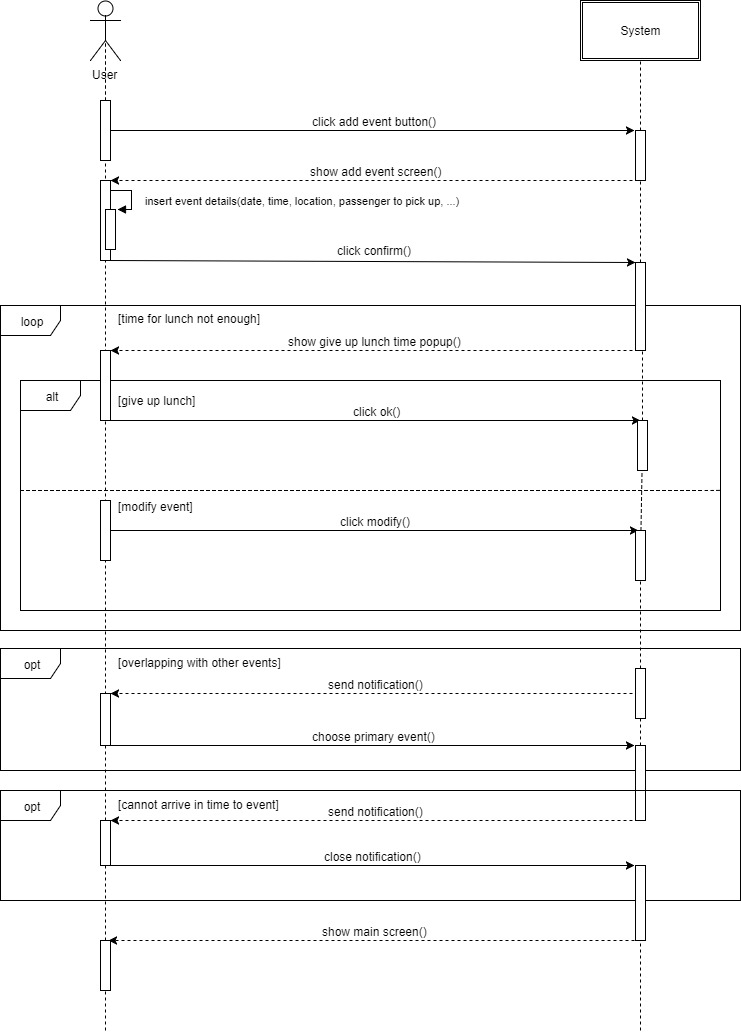
\includegraphics[scale=0.55]{MainMatter/images/sequencediagrams/add}
\captionof{figure}{Sequence diagram of add event use case}
\end{center}

\begin{center}
\def\arraystretch{1.25}
  \begin{tabular}{ | l | p{0.65\textwidth} | }
    \hline
    Name & Delete event from calendar \\ \hline
    Primary Actor & User \\ \hline
    Preconditions & The user wants to delete an event from the calendar of his application. He is already logged in into the service and the system is showing the calendar \\ \hline
    Postconditions & The event is deleted from the calendar and from the database, the system shows again the calendar to the user \\ \hline
    Flow of events  & 1.	The user selects the event he wants to delete \\
					& 2.	The system shows the Event Details screen \\
					& 3.	The user taps on “Modify Event” \\
					& 4.	The system shows Event Edit screen \\
					& 5.	The user clicks on “Delete Event” \\
					& 6.	The system deletes the event from the calendar and from the database, and shows the updated calendar to the user \\
 \hline    
    Exceptions  & 1.	The event overlaps with at least other two events and it is primary \\
 \hline
  \end{tabular}
\captionof{table}{Use case for delete event}
\end{center}

\begin{center}
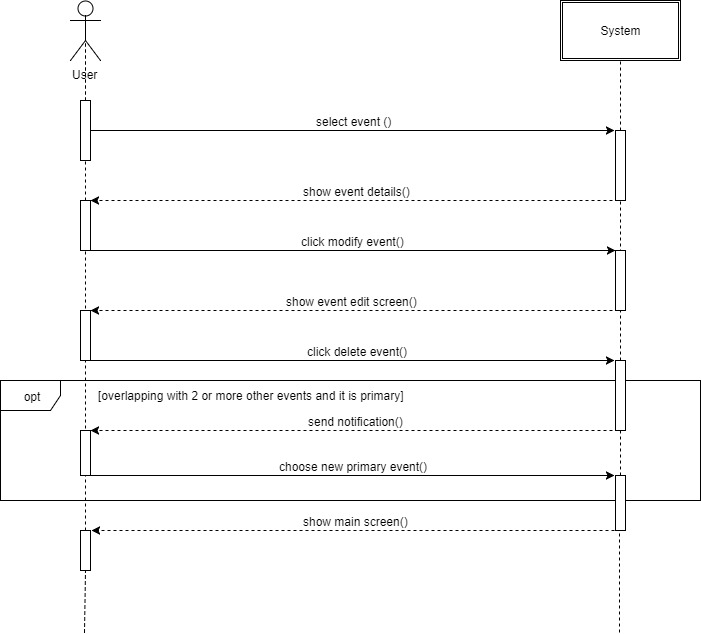
\includegraphics[scale=0.55]{MainMatter/images/sequencediagrams/delete}
\captionof{figure}{Sequence diagram of delete event use case}
\end{center}

\begin{center}
\def\arraystretch{1.25}
  \begin{tabular}{ | l | p{0.65\textwidth} | }
    \hline
    Name & Arrange trip \\ \hline
    Primary Actor & User \\ \hline
    Preconditions & The user wants to buy the tickets to take a trip. He is already logged in into the service and the system is showing the calendar \\ \hline
    Postconditions & The user receives the tickets \\ \hline
    Flow of events  & 1.	The user clicks on “Trips” (the button with the airplane) \\
					& 2.	The system shows the Trips screen \\
					& 3.	The user chooses the event he wants to buy the tickets for \\
					& 4.	The system shows the Trip details screen \\
					& 5.	The user clicks “Buy Now” \\
					& 6.	The system opens a link to buy the ticket and shows the checkout page to the user for every ticket purchasable online \\
					& 7.	The user pays and confirms for all the tickets \\
					& 8.	The system calls the External services that send the tickets to the user  \\
					& 9.	The user communicate to the system that the tickets are bought \\
 \hline    
 	Alternative flow    & 1.	The same operations as above until point 5 \\
						& 2.	The system calls the External services applications that show the checkout screen to the user, for every ticket only purchasable through the proprietary application \\
						& 3.	The user pays and confirms for all the tickets \\
						& 4.	The External services applications send the tickets to user \\
						& 5.	The user communicate to the system that the tickets are bought \\
 \hline
    Exceptions  & 1.	One or more payment failed \\
				& 2.	The user doesn’t confirm payment for one or more tickets \\
 \hline
  \end{tabular}
\captionof{table}{Use case for arrange trip}
\end{center}

\begin{center}
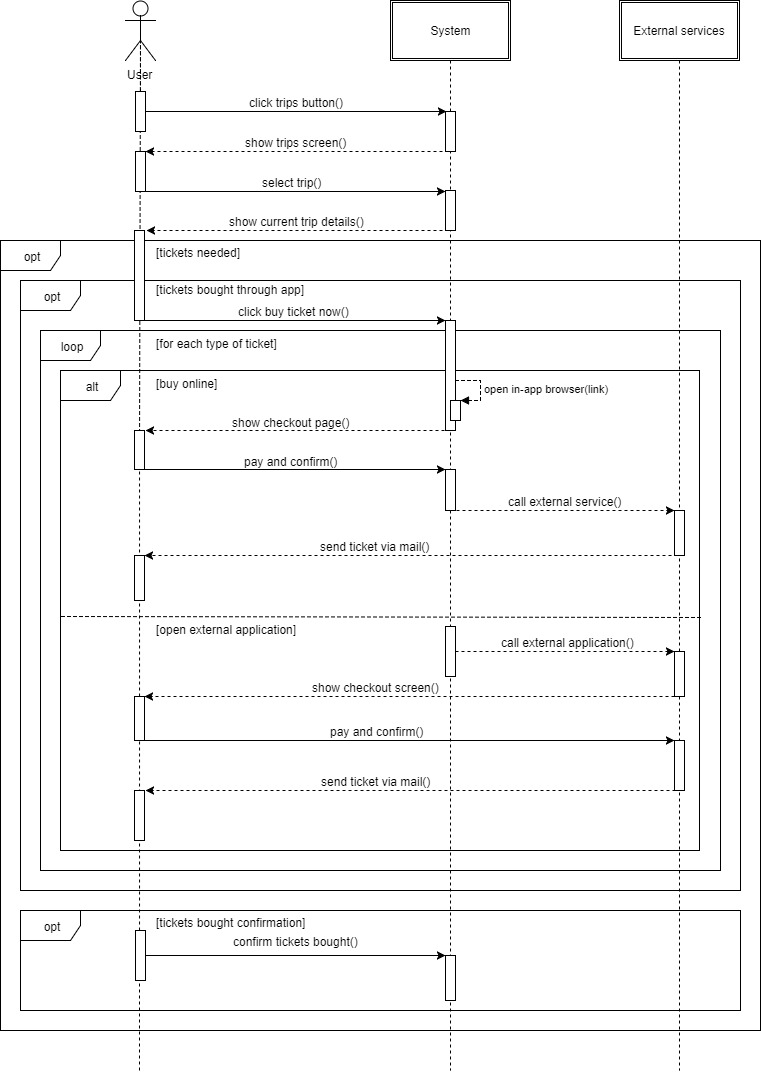
\includegraphics[scale=0.519]{MainMatter/images/sequencediagrams/arrange}
\captionof{figure}{Sequence diagram of arrange trip}
\end{center}

\begin{center}
\def\arraystretch{1.162}
  \begin{tabular}{ | l | p{0.65\textwidth} | }
    \hline
    Name & Manage trip options (customized trip) \\ \hline
    Primary Actor & User \\ \hline
    Preconditions & The user wants to change the modality of one of his trips, choosing to customize it and changing the preferred means of transport. He is already logged in into the service and the system is showing the calendar \\ \hline
    Postconditions & The trip is saved and changed as the user prefers \\ \hline
    Flow of events  & 1.	The user clicks on “Trips” (the button with the airplane) \\
					& 2.	The system shows the Trips screen \\
					& 3.	The user chooses the event he wants to modify \\
					& 4.	The system shows the Trip details screen \\
					& 5.	The user clicks “Modify” \\
					& 6.	The system shows Suggested Trip Choices screen \\
					& 7.	The user select “Customized” \\
					& 8.	The system calculates all available trip options and shows them to the user in the Trip Options screen \\
					& 9.	The user chooses new preferred means of transport \\
					& 10.	The system recalculate all the trip options with the User selection and show them to the user in the Trip Options screen \\
					& 11.	The user chooses his preferred trip option \\
					& 12.	The system shows the Trip details screen \\
					& 13.	The user selects back (the arrow icon) \\
					& 14.	The system shows the Main screen to the user
\\
 \hline
    Exceptions  & 1.	The user chooses to go only by foot but the distance to walk is wider than the one set in the preferences \\
				& 2.	The user chooses to go only by bike, but the time is not inside the interval chosen in the preferences
 \\
 \hline
  \end{tabular}
\captionof{table}{Use case for manage trip options, in the case that the user chooses to customize the trip}
\end{center}

\begin{center}
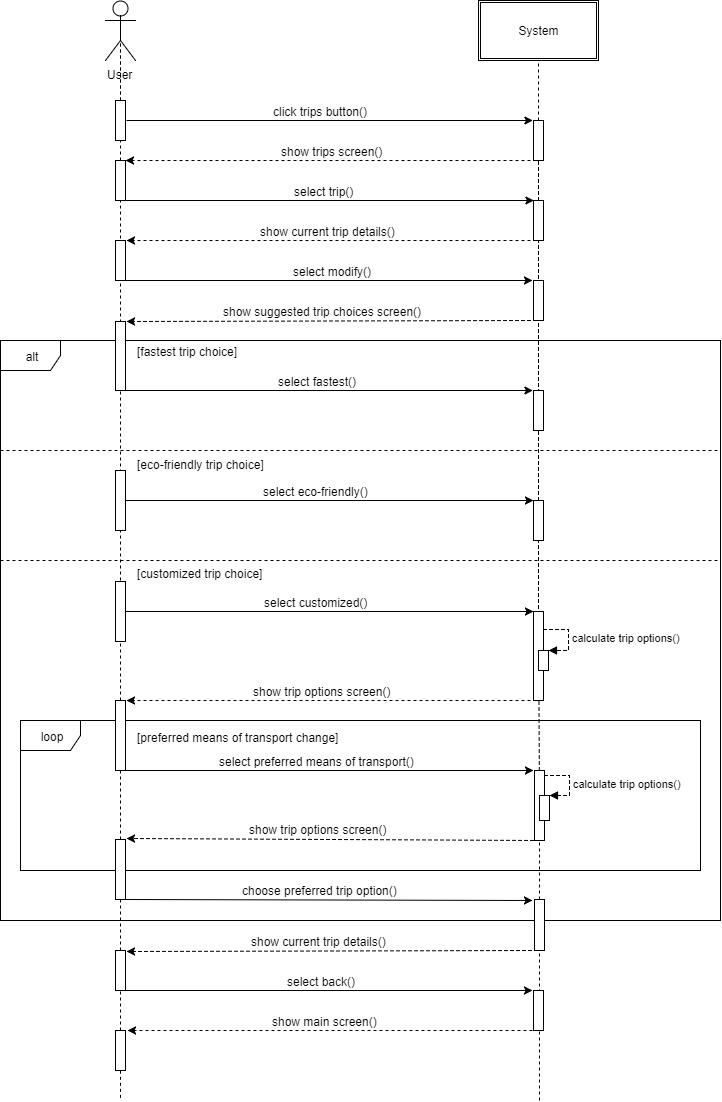
\includegraphics[scale=0.516]{MainMatter/images/sequencediagrams/managetrip}
\captionof{figure}{Sequence diagram of manage trip options}
\end{center}

\begin{center}
\def\arraystretch{1.25}
  \begin{tabular}{ | l | p{0.65\textwidth} | }
    \hline
    Name & Reserve a sharing means of transport \\ \hline
    Primary Actor & User \\ \hline
    Preconditions & The user wants to reserve a sharing means of transport. He is already logged in into the service and the system is showing the calendar \\ \hline
    Postconditions & The user has reserved the means of transport chosen and receives a confirmation via mail \\ \hline
    Flow of events  & 1.	The user clicks on “Trips” (the button with the airplane) \\
					& 2.	The system shows the Trips screen \\
					& 3.	The user chooses the event that is active \\
					& 4.	The system shows the Trip details screen \\
					& 5.	The user clicks on the “Sharing” button \\
					& 6.	The system requests the position of the means of transport to all External Sharing Services and it shows to the user \\
					& 7.	The user chooses a means of transport \\
					& 8.	The system opens the application of the Sharing Service chosen \\
					& 9.	The user reserves the means of transport \\
					& 10.	The Sharing Service application sends a confirmation via mail and shows the means of transport reserved \\
 \hline
    Exceptions  & 1.	The Sharing Service application is not installed on the device \\
				& 2.	The user doesn’t have an account for the Sharing Service

 \\
 \hline
  \end{tabular}
\captionof{table}{Use case for reserve a sharing means of transport}
\end{center}

\begin{center}
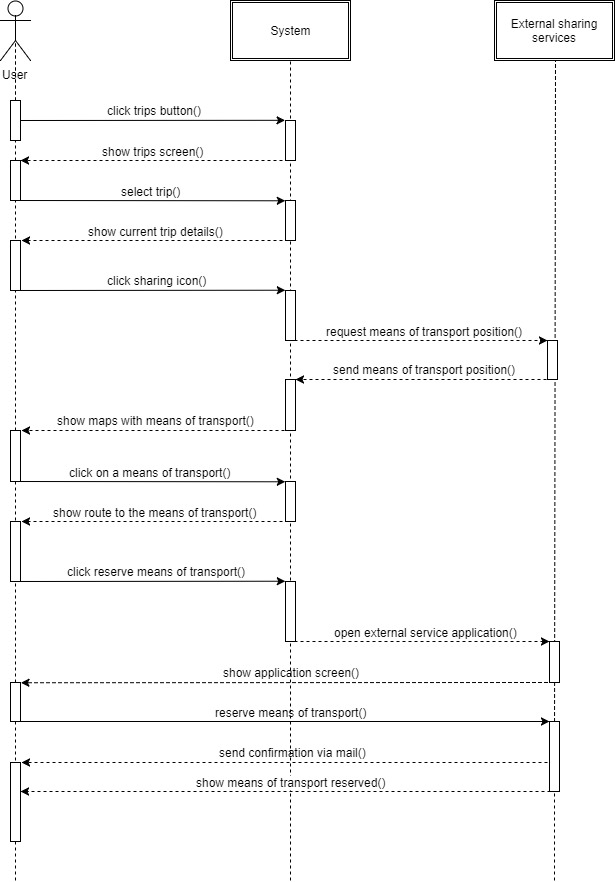
\includegraphics[scale=0.55]{MainMatter/images/sequencediagrams/reservesharing}
\captionof{figure}{Sequence diagram of reserve a sharing means of transport}
\end{center}
\pagebreak
%
%------------------------------------------------------------------------ %
%
\section{Performance Requirements}
\begin{enumerate}
\item The system must support 500 contemporary requests;
\item 90\% of requests must be processed in less than 3 seconds;
\item 100\% of requests must be processed in less than 10 seconds;
\item There’s no limit on the number of users;
\item The system will compute continuously all the travel options for the different users, but must find a free time spot to answer to new requests.
\end{enumerate}
%
% ------------------------------------------------------------------------ %
%
\section{Design Constraints}
%
\subsection{Standards compliance}
This document follows the IEEE Standard 830-1998 [7] for the format of Software Requirements specifications.
%
\subsection{Hardware limitations}
The user will need a smartphone with at least:
\begin{itemize}
\item 3G connection
\item GPS
\item Enough storage on smartphone
\end{itemize}
%
\subsection{Any other constraint}
******************************************************************************************************************************************************
% ------------------------------------------------------------------------ %
%
\section{Software System Attributes}
%
\subsection{Reliability}
The system shall have an availability of 99.95\% (“three and a half nines”). It means that the application will have at most a downtime per year of 4.38 hours.
%
\subsection{Availability}
The system will run 24/7 in order to make the user manage his events and the trips between them whenever he wants. Furthermore any kind of update must not stop the normal running of operations.
%
\subsection{Security}
The main security features of the application are:  
\begin{itemize}
\item All the meetings and the trips must be kept private.
\item Enable SSL/TLS encryption protocol for Client-Server communication to protect from internal and external threats, depending on user’s network configuration. Enabling SSL/TLS ensures the confidentiality, authentication, and integrity of session data.
\item Insecure communication channels will lead to a refuse for the client’s request.
\item Passwords must be encrypted, hashed and salted before they could be stored in the databases.
\item Users can access in reading or in writing on only a limited set of data.
\end{itemize}
%
\subsection{Maintainability}
The application code will be well documented to let future developers understand how it work and to make them able to modify it.
%
\subsection{Portability}
The application will be available for the two most common mobile operating systems: Android and iOS.
% ------------------------------------------------------------------------ %


% -----------------------------END------------------------------------- %

%
% ------------------------------------------------------------------------ %
% !TEX encoding = UTF-8
% !TEX TS-program = pdflatex
% !TEX root = ../Project.tex
% !TEX spellcheck = en-EN
% ------------------------------------------------------------------------ %
%
% ------------------------------------------------------------------------ %
% 	CHAPTER TITLE
% ------------------------------------------------------------------------ %
%
\chapter{Formal Analysis}
%
\label{cap:formalanalysis}
%
% ------------------------------------------------------------------------ %
%
% -----------------------------END------------------------------------- %
%
% ------------------------------------------------------------------------ %
% !TEX encoding = UTF-8
% !TEX TS-program = pdflatex
% !TEX root = ../Project.tex
% !TEX spellcheck = en-EN
% ------------------------------------------------------------------------ %
%
% ------------------------------------------------------------------------ %
% 	CHAPTER TITLE
% ------------------------------------------------------------------------ %
%
\chapter{Effort Spent}
%
\label{cap:effortspent}
%
% ------------------------------------------------------------------------ %

\begin{center}
\def\arraystretch{1.25}
  \begin{tabular}{ | l | c | c | c |}
    \hline
    Date & A. Aimi & R. Bigazzi & F. Collini \\ \hline
    03/10/17 & 4h & 5h & 4h \\
    05/10/17 & & 1/2h& \\
    06/10/17 & 2h & & \\
    07/10/17 & 1h & 1h & 1h\\
    08/10/17 & & & 2h\\
    09/10/17 & 4h & 2h & \\
    12/10/17 & 3h & 3h & 3h \\
    14/10/17 & & 1h & 1h \\
    15/10/17 & 1,5h & 1/2h & \\
    18/10/17 & 2h & 2h & 2h \\
    19/10/17 & & & 3h\\
    20/10/17 & 2h & & \\
    23/10/17 & 4h & 4h & 4h \\
    24/10/17 & & 2h & 1h \\
    25/10/17 & & 3h & 2h\\
    26/10/17 & 1h & 2h & \\
    27/10/17 & 2,5h & 1/2h & 2,5h\\
    28/10/17 & 5h & 8h & 6h \\
    29/10/17 & 6h & 6h & 6h \\ \hline
    Tot & 38h & 40,5h & 37,5h \\ \hline
  \end{tabular}
\captionof{table}{Hours of work spent by the authors of the document}
\end{center}
%
% -----------------------------END------------------------------------- %
%
% ------------------------------------------------------------------------ %
% !TEX encoding = UTF-8
% !TEX TS-program = pdflatex
% !TEX root = ../Project.tex
% !TEX spellcheck = en-EN
% ------------------------------------------------------------------------ %
%
% ------------------------------------------------------------------------ %
% 	CHAPTER TITLE
% ------------------------------------------------------------------------ %
%
\chapter{Formal Analysis}
%
\label{cap:formalanalysis}
%
% ------------------------------------------------------------------------ %
%
\section{Modeling}
\lstinputlisting[language=alloy]{MainMatter/alloy.als}
%
% ------------------------------------------------------------------------ %
%
\begin{center}
\vspace{10mm}
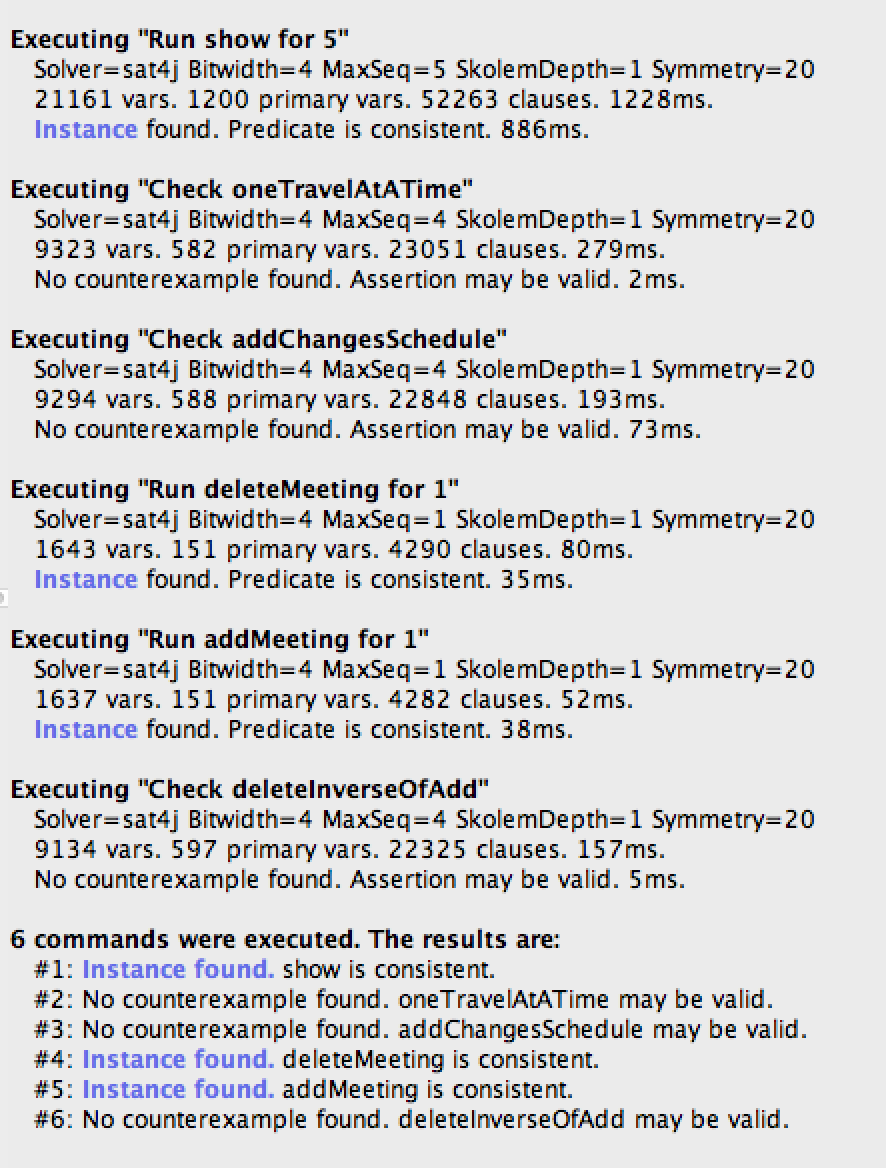
\includegraphics[scale=0.8]{MainMatter/images/alloy/results}
\captionof{figure}{Result of Alloy Analyzer}
\end{center}
%
\begin{landscape}
\section{World generated}
\begin{center}
\thispagestyle{empty}
\makebox[\textwidth][c]{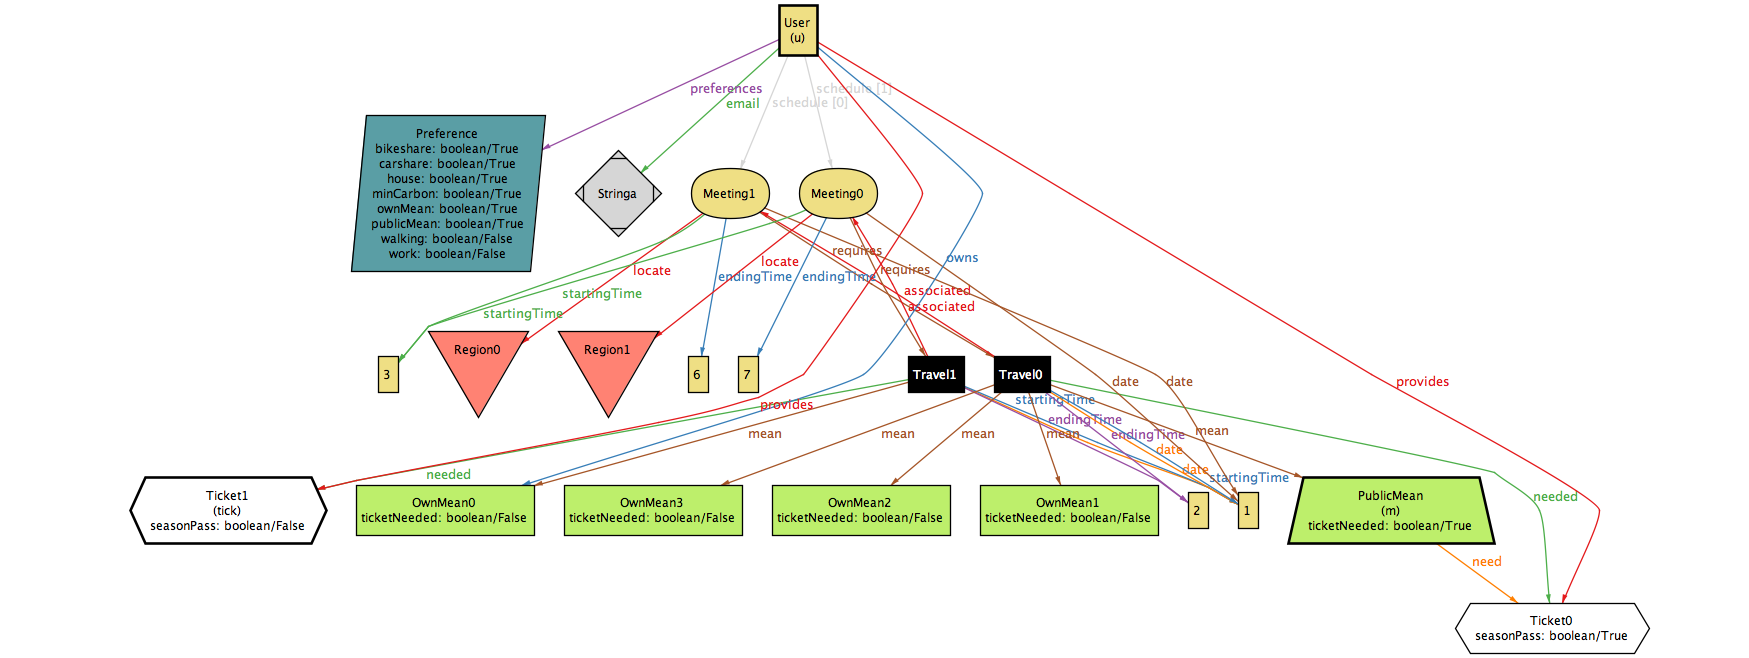
\includegraphics[width=2.3\textwidth]{MainMatter/images/alloy/world}}
\captionof{figure}{World generated}
\end{center}
\end{landscape}
%
\section{Alloy vs UML}
What we’ve modelled of the UML in alloy: \\
The goal of modelling in alloy is to describe some aspect of the system (but not the entire system), constrain it to exclude ill-formed examples and check properties about it.
The section in UML concerning the external companies connected to Travlendar+, for instance the ones which can provide tickets or that can offer sharing systems, is not modelled in Alloy cause we assume that they will behave correctly in our system thanks to the agreements they took with us.
We are also didn’t model time because it’s not useful in the model, but we will care about it in other portions of the project analysis. The time break will not be modelled and also the fact that the application will not advise trips by bike or foot on late hours.
%
% -----------------------------END------------------------------------- %
%
% ------------------------------------------------------------------------ %
% !TEX encoding = UTF-8
% !TEX TS-program = pdflatex
% !TEX root = ../Project.tex
% !TEX spellcheck = en-EN
% ------------------------------------------------------------------------ %
%
% ------------------------------------------------------------------------ %
% 	CHAPTER TITLE
% ------------------------------------------------------------------------ %
%
\chapter{Effort Spent}
%
\label{cap:effortspent}
%
% ------------------------------------------------------------------------ %
%

\begin{center}
\def\arraystretch{1.25}
  \begin{tabular}{ | l | c | c | c |}
    \hline
    Date & A. Aimi & R. Bigazzi & F. Collini \\ \hline
    15/11/17 & & 1,5h & 1,5h\\
    17/11/17 & & 3h & 4h \\
    18/11/17 & 3h & 3h & 5h \\
    19/10/17 & 2h & & 2h \\
    20/10/17 & 2h & 2h & 2h \\
    21/10/17 & 3h & 1h & 3h\\
    22/10/17 & 6h & 4h & \\
    23/10/17 & 3h & 2h & 3h\\
    24/10/17 & 4h & 4h & 4h \\
    25/10/17 & 7h & 7h & 5h \\
    26/10/17 & 6h & 6h & 6h \\ \hline
    Tot & 36h & 33,5h & 35,5h \\ \hline
  \end{tabular}
\captionof{table}{Hours of work spent by the authors of the document}
\end{center}
%
% -----------------------------END------------------------------------- %
%
%\appendix
%
%\input{MainMatter/Appendix}
%
% ------------------------------------------------------------------------ %
% 	BACKMATTER
% ------------------------------------------------------------------------ %
%
%\backmatter
%
%\input{BackMatter/Bibliography}
%
% ------------------------------------------------------------------------ %
% 	END DOCUMENT
% ------------------------------------------------------------------------ %
%
\end{document}
%
% ------------------------------------------------------------------------ %